\documentclass[a4paper,12pt]{article}

\usepackage{amsmath,amssymb,amsthm,tikz}
\usetikzlibrary{calc,arrows.meta}
\usepackage[margin=20mm]{geometry}
\usepackage{hyperref}
\usepackage{xcolor}

\setlength{\parindent}{0pt}
\setlength{\columnsep}{1cm}

\begin{document}

%\twocolumn

\thispagestyle{empty}

\begin{center}
{\Large Sample Assignment 9}\\
%{\Large Published on 2020-11-08,}\\
{\em Not graded} 
\end{center}

\noindent


\vspace{10pt}
{\bf Pseudocode for Quicksort}. This variant of Quicksort
uses the leftmost element of the input area as a pivot. 
It is the same as
we have in the lecture slides, but may differ from 
some other Quicksort flavors (randomized etc.) that you may encouter
in other sources.

\[
\begin{array}{rl}
 & \text{\textsc{Quicksort}}(A[\ell\;\ldots\;r]):\\
1 & \text{\textbf{if\ }} l<r:\\
2 & \hspace{.5cm} i = \ell \;\;\;\;\;\;\;\;\; \textcolor{teal}{\text{\em ($i$ increases from the left and searches elements $\geq$ than pivot)}}\\
3 & \hspace{.5cm} j = r+1	\;\; \textcolor{teal}{\text{\em ($j$ decreases from the right and searches elements $\leq$ than pivot.)}}\\	
4 & \hspace{.5cm} v = A[\ell] \;\;\;\; \textcolor{teal}{\text{\em ($v$ is the pivot.)}}\\
5 & \hspace{.5cm} \text{\textbf{while\ }} i<j:\\
6 & \hspace{1.0cm} i = i+1\\
7 & \hspace{1.0cm} \text{\textbf{while\ }} \textcolor{red}{i<r} \text{\textbf{\ and\ }} A[i]<v:\\
8 & \hspace{1.5cm} i = i+1\\
9 & \hspace{1.0cm} j = j-1\\
10 & \hspace{1.0cm} \text{\textbf{while\ }} \textcolor{red}{j>\ell} \text{\textbf{\ and\ }} A[j]>v:\\
11 & \hspace{1.5cm} j = j-1\\
12 & \hspace{1.0cm} A[i] \leftrightarrow A[j] \;\; \textcolor{teal}{\text{\em (Undo the extra swap at the end)}}\\
13 & \hspace{0.5cm} A[i] \leftrightarrow A[j] \;\; \textcolor{teal}{\text{\em (Undo the extra swap at the end)}}\\
14 & \hspace{0.5cm} \textcolor{red}{A[j]} \leftrightarrow A[\ell] \;\; \textcolor{teal}{\text{\em (Move pivot to its proper place)}}\\
15 & \hspace{0.5cm} \text{\textsc{Quicksort}}(A[\ell\;\ldots\;j-1])\\
16 & \hspace{0.5cm} \text{\textsc{Quicksort}}(A[j+1\;\ldots\;r])\\
\end{array}
\]


\vspace{5pt}
{\bf (A)}
Run this pseudocode for one invocation $\text{\textsc{QuickSort}}(A[0..11])$, 
where the table to sort is the following: 
$$13, 0, 23, 1, 8, 9, 29, 16, 8, 24, 6, 11$$
Draw the state of the array every time you swap two 
elements (i.e.\ execute $A[k_1] \leftrightarrow A[k_2]$ for any $k_1,k_2$).

\vspace{5pt}
{\bf (B)}
Continue with the first recursive call of $\text{\textsc{QuickSort}}()$
(the original call $\text{\textsc{QuickSort}}(A[0..11])$ is assumed to be the
$0^{\text{th}}$ call of this function). 
Draw the state of the array every time you swap two 
elements. 


\vspace{5pt}
{\bf (C)} Decide which is the second recursive call of 
$\text{\textsc{QuickSort}}()$ and draw the state 
of the array every time you swap two elements. 
Show the end-result 
after this second recursive call at the very end.


\newpage
{\bf Solution.}\\
{\em Your answer can be simple lists of numbers (without any grid lines or additional 
markings). Just try to keep the lists of numbers aligned. 


\vspace{5pt}
{\bf (A)}

\begin{figure}[!htb]
\center{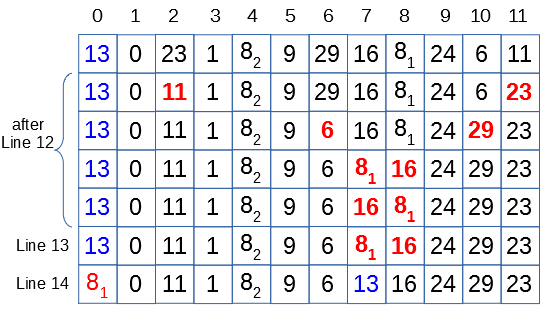
\includegraphics[width=4in]{assignment09-quicksort/arrays-part1.png}}
\caption{\label{fig:arrays-part1} Swaps during the $0^{\text{th}}$ call.}
\end{figure}



\vspace{5pt}
{\bf (B)} Since this example contains two elements equal to $8$, 
we added subscripts to them (to show clearly, where every one is being swapped). 
As integer numbers they are fully identical to the Quicksort algorithm. 
(Still, the Quicksort algorithm does redundant swaps on them.)


\begin{figure}[!htb]
\center{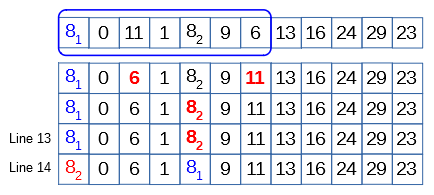
\includegraphics[width=4in]{assignment09-quicksort/arrays-part2.png}}
\caption{\label{fig:arrays-part2} Swaps during the first recursive call.}
\end{figure}


\vspace{5pt}
{\bf (C)} Notice that the second recursive call happens within the 
first recursive call (sorting the left side of the left half). 


\begin{figure}[!htb]
\center{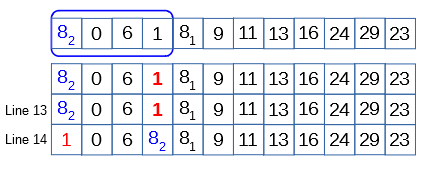
\includegraphics[width=4in]{assignment09-quicksort/arrays-part3.png}}
\caption{\label{fig:arrays-part3} Swaps during the second recursive call.}
\end{figure}





\end{document}



